% compile by  pdflatex blog; biber blog
% GitHub cvitanov/reducesymm/dasgroup/birdtracks.tex

% Predrag  created              Aug 7 2014
% notes for birdtracks.eu



\chapter{Birdtracks}
\label{c-birdtracks}


Enter here notes of general group-theoretic interest, perhaps for inclusion
into revisions of \wwwgt. The notes are in
\\
\HREF{https://github.com/cvitanov/reducesymm/}
{GitHub.com/cvitanov/reducesymm}. If you download it
\\
\texttt{> cd dasgroup/} \\
\texttt{> pdflatex blog} \\
For anything
technical, please do not email me, but let me give you permissions to edit
this GitHub repository. Then you can  edit directly into the GitHub version,
and let me know by email to \\
\texttt{dasgroup@mail.gatech.edu}\\
when you have \texttt{git push}ed something new to the server.



\section{Notes on Alcock-Zeilinger and Weigert}
\label{s-AlcZei16}

\newcommand{\FPic}[1]{\raisebox{-0.4\height}{\hspace{-0.27mm}\includegraphics{#1}\hspace{-0.27mm}}}
\newcommand*\circled[1]{\tikz[baseline=(char.base)]{
            \node[shape=circle,draw,inner sep=2pt] (char) {#1};}}
\newcommand{\diagram}[2][{}]{\pbox{\textwidth}{\includegraphics[#1]{{#2}}}}
\newcommand{\SUN}{\mathsf{SU}(N)}
\newcommand{\MixedPow}[2]{V^{\otimes
    #1}\otimes\left(V^*\right)^{\otimes #2}}
\newcommand{\Pow}[1]{V^{\otimes #1}}
\newcommand{\DAlg}[1]{\left(V^*\right)^{\otimes #1}}
\newcommand{\Lin}[1]{\mathrm{Lin}\left( #1 \right)}
\newcommand{\API}[1]{\mathsf{API}\left( #1 \right)}
\newcommand{\InvAlg}[1]{A\left[ S_{#1} \right]}
\newcommand{\Rsim}{\stackrel{\mathcal{R}}{\sim}}

\begin{description}
  \item[2016-12-08 Predrag to Heribert:]
My
\HREF{http://chaosbook.org/~predrag/papers/preprints.html\#FiniteFieldTheo}
{``finiteness conjecture''} is based on the observation that if internal
photons are collected into gauge invariant sets, each set contributes a
small, finite amount to what (off-mass shell) is usually assumed to be an
asymptotic series.
A gauge invariant set contributing to $(m+m'+k)$th order consists of $m$
photon ``strands" attached to the incoming electron, $m'$ photon ``strands"
attached to the outgoing electron, and $k$ photon ``strands" crossing the
external photon vertex. I do not have a direct method for evaluating a gauge
set; instead, it takes a few years and a PhD thesis to evaluate these sets.

These photon ``strands" have infrared divergences in individual diagrams,
but as one is evaluating the magnetic moment, their sums do not.

Do you envision using Wilson lines formulation possibly accounting for clouds
of soft photons crossing a QED vertex? Is there a direct calculation one
could do without perturbatively expanding the Wilson lines to the usual
individual multi-photon Feynman diagrams?

  \item[2016-12-02 Predrag]
My notes  on Alcock-Zeilinger and Weigert are in\\
\HREF{https://github.com/cvitanov/reducesymm/}
{GitHub.com/cvitanov/reducesymm/dasgroup/}.

  \item[2016-11-30 Predrag]
Your Sect.~4.2 Proof of Theorem 3 \emph{(generalized propagation rules)}
seems not to need Young tableaux to work. A streamlined derivation might be
to prove it for an individual transposition, the assemble whatever operator
you need from transpositions?

  \item[2016-12-02 Predrag]
You might consider folding your Mathematica codes into
\texttt{FormTracer}\rf{CyMiSt16} see \refsect{s-code}, entry of {\bf
[2016-12-10]}.

  \item[2016-11-30 Predrag]
Skype session with Heribert and Judy, about their 3 birdtracking preprints.
Got through the first one\rf{AlcZei16-1}.

\end{description}

\subsection{Physics motivation}
\label{s-AlcZei16-HEP}

% Physics motivation:


(read up on Larry McLarren propaganda)

Applications of these
tools in a QCD context where factorization invariably involves color
singlet projections of Wilson line correlators, see
several fields with possible
applications:

Marquet and Weigert\rf{MarWei10} {\em New observables to test the {Color
Glass Condensate} beyond the large-{$N_c$} limit}

Weigert\rf{Weigert03}
{\em Non-global jet evolution at finite {$N_c$}}

Falcioni \etal\rf{FGHMW14}
{\em Multiple gluon exchange webs}

Bomhof \etal\rf{BoMuPi06}
{\em The construction of gauge-links in arbitrary hard processes}

Since $\SUN$ is the gauge group of QCD, \Ypo s come into play through the
theory of invariants, which relates the irreducible representations of $\SUN$
over $\Pow{n}$ to the Young tableaux of size $n$\rf{Fulton97,Tung1985na}.
The lack of Hermiticity of \Ypo s  disqualifies them from the application to
QCD calculations: for applications the operators need to be Hermitian (hence
\refrefs{KeppSjo14,AlcZei16-2}) and all singlets are accounted for (hence
\refref{AlcZei16-4}).

Functional evolution evolution equation  for QCD cross sections in high
energy limit (Bjorken $x$ less than $10^{-2}$), as you push up energy make
more and more soft gluons, making the system highly nonlinear. Parton model
picture breaks down. BFKL pomeron equation is in Bjorken $x$, but distributions go
exponentially large; Weigert contributed to formulating the nonlinear
version.

{\em Color Glass Condensate} (within the standard model, only QCD does it):
\\

The Balitsky-\-JIMWLK (Jalilian-\-Marian-\-Iancu-\-McLerran-\-Weigert-\-Leonidov-\-Kovner)
is a tool to calculate the energy dependence of QCD observables at high
energies. Gluon  distribution  in  a  proton  as  a  function  of impact
parameter and rapidity can be described by the functional Langevin version of
the JIMWLK renormalization group equation.

The meson production cross-sections contain four point correlators
whose evolution follows from the JIMWLK framework. The four point correlators
are here computed beyond the large-Nc limit.

$N_c$ limit breaks gauge invariance, Weigert restores it minimally on the
level of Wilson lines.

Needed for Wilson lines, in jet-like situations (scattering experiment jet
observables) need to get all color singlets, SU(n).

Only thing that can happen are color rotations (that's where Wilson lines,
driven by the soft gluons, come in), JIMWLK gives effective field theory for
expectation values of these Wilson lines, globally colorless states.

Came from correlators of Wilson lines, needed to get all color singlets for
$\SUn{n}$.

The theory of invariants,
relates the irreducible representations of $\SUN$ over $\Pow{n}$
to the Young tableaux of size $n$, see \refrefs{Fulton97,Tung1985na}
and other standard textbooks.


\subsection{Simplification rules for birdtrack operators}
\label{s-AlcZei16-1}

Notes on Alcock-Zeilinger and Weigert\rf{AlcZei16-1}.

They credit Young\rf{Young1933} for introducing \Ypo s,
and refer to Tung\rf{Tung1985na} as the standard reference for them.

\subsubsection{%         \medskip\noindent Sect.~\emph{
2 Notation, conventions and known results}

The direction of the arrow on the index lines of a birdtrack encodes whether
the line acts on the vector space $V$ (arrow pointing from right to left) or
its dual $V^*$ (arrow pointing from left to right)\rf{AlcZei16-3}.
In general birdtracks represent primitive invariants of $\SUN$ over a mixed
algebra $\MixedPow{m}{n}$, where $V^*$ is the dual vector space of $V$.
Here only birdtracks acting on a space $\Pow{m}$ are considered (never on the
dual). As all arrows go from right to left, they can be dropped.

The permutations of $\textrm{S}_n$ are the \emph{primitive invariants}\rf{AlcZei16-3}
(of $\SUN$ over $\Pow{n}$).
The real subalgebra of $\Lin{\Pow{n}}$ that is spanned by these primitive
invariants is denoted $\API{\SUN,\Pow{n}}\subset\Lin{\Pow{n}}$.
{API} stands for ``\api.''
One
distinguishes

\begin{description}
  \item[Semi-standard irregular tableaux]
Each number
appears \emph{at most once} within a tableau.
  \item[Young tableaux]
The boxes are top- and left-aligned.
The numbers in the boxes to increase within each row from left to right and
within each column from top to bottom.
  \item[Amputated tableaux]
The \emph{column-amputated tableau} is obtained by removing all columns
which do not overlap with the given row.
The \emph{row-amputated tableau}  is obtained by removing all rows which do
not overlap with the given column.
\end{description}

$A\subset B $ denotes that a \emph{Hermitian} projection operator $A$
projects onto a subspace completely contained in the image of a projection
operator $B$, \ie, $A\subset B$ if and only if
\beq
  \label{eq:OperatorInclusion1}
  A \cdot B = B \cdot A = A
\,.
\eeq
This simplification rule breaks down for the standard Young projection
operators whenever they are not Hermitian.

The main result of this paper are the two kinds of simplification rules
(cancellation or propagation) for birdtrack operators $O$ comprised of
symmetrizers and antisymmetrizers.

\subsubsection{%         \medskip\noindent Sect.~\emph{
3 Cancellation rules}

(1) Cancelation rules : Rules to determine whether certain symmetrizers or
antisymmetrizers within an operator $O$ are redundant, and thus can be
\emph{cancelled} from an operator. They can make a long expression
significantly shorter, and thus easier to work with.

The two main cancellation rules are
the {\em cancellation of wedged \Ypo s}, and
the {\em cancellation of wedged ancestor-operators}.

\subsubsection{%         \medskip\noindent Sect.~\emph{
3.1 Cancellation of wedged \Ypo s}

Theorem 1. Outside S and A, inside a \Ypo\

The example that starts with Eq.~(17), goes to the top of the page 10
motivates the general algorithm to remove inner symmetrizers.

The points 1. 2. and 3. are general, not just for this particular tableaux,
hence:

Corollary~1. {\em Cancellation of wedged ancestor-operators}:
can always get rid of an interior \Ypo.

\subsubsection{%         \medskip\noindent Sect.~\emph{
3.2 Cancellation of factors between bracketing sets}

Cancelation rules :
move sets of symmetrizers or antisymmetrizers
through certain parts of the operator.
\\

\noindent\emph{horizontal permutations} of $\Tilde{\Theta}$:
$\mathbf{h}_{\Tilde{\Theta}}$ is the subset of all permutations in
  $\textrm{S}_n$ that only operate within the rows of $\Tilde{\Theta}$; i.e. that do
  not swap numbers across rows. \\
\emph{vertical permutations} of $\Tilde{\Theta}$:
  $\mathbf{v}_{\Tilde{\Theta}}$ is the subset of permutations in $\textrm{S}_n$
  that only operate within the columns of $\Tilde{\Theta}$.
\\

(I am too lazy to work through Tung's Lemma IV.5)
\\


Corollary~2. {\em Cancellation of parts of the operator}
One can always get rid of an inner \Ypo. They lack explicit formula
for the constants; so make sure non-zero, at the end evaluate
the overall constant by other means (projection operator conditions).

Outer $\mathbf{A}_{\Theta}$ and $\mathbf{S}_{\Theta}$ belong to the same
\Ypo, see Eq.~(23): there exists a (possibly vanishing)
constant $\lambda$ such that
  \begin{equation}
    \label{eq:Cancel-General-O}
\mathbf{S}_{\Theta} \; M \; \mathbf{A}_{\Theta} =
\lambda \cdot Y_{\Theta}
\ .
  \end{equation}

The rest of the section  ensures that the constant is non-zero. It's quite of
bit of work, I skipped it (unless they want me to work through some of it).

\subsubsection{%         \medskip\noindent Sect.~\emph{
Dimensional zeroes}

If any of the antisymmetrizers exceed the length $N$ one has a
\emph{dimensional zero}. So one needs to assume $N$ is high enough.
It should work out once the calculation is done - every polynomial
will have zeros for $N$ to small for a given tableaux.


\subsubsection{%         \medskip\noindent Sect.~\emph{
4 Propagation rules}

rules when things commute

(2) {Propagation rules} :
when it is possible to commute (\emph{propagate}) a symmetrizer through an
antisymmetrizer (or vice versa)? Then the cancellation rules might be
applied, or features of a particular operator $O$, such as its Hermiticity
can be made explicit. The answer:
\[
O =\; \scalebox{0.75}{\FPic{mOpsO}} \; = \;
\scalebox{0.75}{\FPic{mOpsOHermitean}} \; = \;
\scalebox{0.75}{\FPic{mOpsOHC}} \; = O^{\dagger}
\,.
\]
It something I had used in the birdtracks.eu book in inchoate manner - they
make it into a precise algorithm.


Example Eq.~(45) is a bit tough

Example Eq.~(48) through Eq.~(50) is easy.



rest of the section is ``Q. when you can commute?''

A. If can get rectangular tableaux, then it commutes

In particular, works also for semi-standard irregular tableaux,
\\
Theorem~3 {\em (generalized propagation rules)}

Eq.~(57) tells it


\subsubsection{%         \medskip\noindent Sect.~\emph{
4.1 Proof of Theorem 2 (generalized propagation rules)}

Proof is long and painful - I did not go through it. Should I?

\subsubsection{%         \medskip\noindent Sect.~\emph{
5 Conclusion}

Keppeler and Sj{\"o}dahl\rf{KeppSjo14} were the first to offer a simple
method to construct Hermitian operators: their iteration is easy to
understand, and the proofs of hermiticity are simple proofs. However, in
practice, the algorithm is inefficient - the expression balloon quickly.

The methods of this paper are also recursive, but with the recursion cut down
drastically. The gain is illustrated by Fig.~5.2 in the paper, here
reproduced as \reffig{fig:MOLDAdvantage}.


\subsection{Compact Hermitian \Ypo s}
\label{s-AlcZei16-2}

Notes on Alcock-Zeilinger and Weigert\rf{AlcZei16-2}.

\Ypo s are (1) idempotent, (2) orthogonal and (3) complete.
But, as the symmetrizers and antisymmetrizers comprising a given Young
tableau do not necessarily commute,  \Ypo s are in general not Hermitian.

Keppeler and Sj{\"o}dahl\rf{KeppSjo14} were first to construct Hermitian
versions of Young projection operators in the birdtrack formalism, by an
iterative algorithm. However, the KS-operators soon become unwieldy and thus
impractical to work.

The construction algorithm presented here,
based on the simplification rules of \refref{AlcZei16-2},
leads to drastically more compact and explicitly Hermitian
expressions for the projection operators than the
KS-algorithm\rf{KeppSjo14}; an example is given
in \reffig{fig:MOLDAdvantage}.

\begin{figure}% [H]
%\newlength\foo
%\settototalheight\foo{\resizebox{\textwidth}{!}{%
%  \diagram[height=.15cm]{MOLDAdvantageEx2}
%}}
  \begin{center}
\resizebox{\textwidth}{!}{%
\begin{tikzpicture}[every node/.style={inner sep=1pt, outer sep=0pt}]
\node (KS) {\diagram[height=.15cm]{MOLDAdvantageEx2}};
\node (short) at ($(KS) +(0,-0.6cm)$)
      {\diagram[height=.15cm]{Simple-KS}};
\node (MOLD) at ($(short) +(0,-0.6cm)$)
      {\diagram[height=.15cm]{MOLDAdvantageEx4}};
\draw[-{stealth}, line width=0.25pt] (KS) to (short);
\draw[-{stealth}, line width=0.25pt] (short) to (MOLD);
\node[scale=0.4] (Cancel) at ($(KS) +(0.7,-0.3cm)$) {Cancellation
  rules};
\node[scale=0.4] (Propagate) at ($(short) +(0.7,-0.3cm)$) {Propagation rules};
\end{tikzpicture}
}
  \end{center}
\caption{
(top)
A Hermitian birdtrack obtained by the iterative KS-algorithm\rf{KeppSjo14}.
Blow it up on the screen to see the details.
(middle)
The much shorter version obtained by application of the cancellation rules.
(bottom)
The explicitly symmetric (Hermitian) version achieved via the propagation
rules.
}
\label{fig:MOLDAdvantage}
\end{figure}


Repeated here are most of the Keppeler and Sj{\"o}dahl\rf{KeppSjo14} {\em
Hermitian \Ypo s}. Keppeler and Sj{\"o}dahl used iterative methods, see
\refref{AlcZei16-2} bottom p.~18


Eq.~(53) not obvious it is symmetric - \rf{AlcZei16-1} gives simplification rules,
dramatic simplification, see Fig.~5.2

\subsubsection{
%\subsubsection{%         \medskip\noindent Sect.~\emph{
3.3 KS Construction principle for Hermitian \Ypo s}


provides a direct route to bottom Fig.~5.2, paper proves that it really works

\Ypo s not being Hermitian has strange consequences.
Eq.~(12) not true, but for the Hermitian ones it is true.

MOLD algorithm yields directly \reffig{fig:MOLDAdvantage}, without going through KS first.


\subsection{Transition operators}
\label{s-AlcZei16-3}

Notes on Alcock-Zeilinger and Weigert\rf{AlcZei16-3}.

The simplification rules of \refref{AlcZei16-2}
allow here a construction of transition operators between (Hermitian) Young
projection operators corresponding to equivalent irreducible representations
of $\SUN$, and an orthogonal basis for the algebra of invariants on
$\Pow{m}$.


completes the picture, the full algebra of invariants

\subsubsection{%         \medskip\noindent Sect.~\emph{
3 Young projection and transition operators}

gives the counting argument that the number of primitive invariants
equals the sum of diagonal operators and transition operators.

\subsubsection{%         \medskip\noindent Sect.~\emph{
5.2 A full orthogonal basis for {\api}}

write Clebsch, as in Eq.~(71)

Eq.~(73) transition operator between equivalent representations

they are unitary if restricted on the representations (top p 21)

together with the hermitian, they give you the full unitary basis

In Eq.~(55a) algebra is decomposed into subalgebras,
Eq.~(55b) is as simple as can be.

Eq.~(63) is non-Hermitian version

see and compare Fig.~2 (non Hermitian) and Fig.~3: (hermitian)
same as birdtracks.eu, but without the transition operators.

Dimension of the algebra goes factorially, so algorithm works up to 8 or 9
(all algebra in Mathematica, up to 8 on the laptop).

\subsection{Singlets}
\label{s-AlcZei16-4}


Notes on J. Alcock-Zeilinger and H. Weigert\rf{AlcZei16-4}.

This paper says that these projection operators give you all singlets.

The orthogonal basis of \refref{AlcZei16-3} is used to form a basis for the
singlet states necessary to determine all color neutral Wilson line
correlators. This has applications in  QCD, such as \refref{MarWei10}
and

Lappi \etal\rf{LRRW16}
{\em {JIMWLK} evolution of the odderon}

\subsection{quarks$~\times~$antiquarks}
\label{s-AlcZei16-qantiq}
see note of {\bf 2019-05-01} below.

\section{Notes on Keppeler and Sj{\"o}dahl}
\label{s-KeppSjo14}

\begin{description}

\item[2014-07-20 PC] More birdtracking - a construction of orthogonal
(Hermitian) projection operators:

\HREF{https://plus.google.com/111710245682175604723}
{Stefan Keppeler} and Malin Sj{\"o}dahl\rf{KeppSjo14} {\em Hermitian \Ypo s}

Sj{\"o}dahl\rf{Sjodahl13,SjoKep13} {\em Tools for calculations in color
space}, Malin.Sjodahl@thep.lu.se

Sj{\"o}dahl \etal\ discuss decomposition into multiplet
  bases\rf{SjoTho15} and recursion relations\rf{DuSjoTho15}.

\item[2018-10-13 PC]
Sj{\"o}dahl's student Thor{\'e}n has Masters\rf{Thoren14} and Phd
Thesis\rf{Thoren18}
{\em Multiplet Bases, Recursion Relations and Full Color Parton Showers}.

Paper I, \refref{SjoTho15}, concerns the decomposition of QCD color structures
into multiplet bases, using Wigner 3j and 6j coefficients. A strong constraint
is put on the required Wigner coefficients for leading order and
next-to-leading order QCD amplitudes. The required Wigner coefficients for up
to six external gluons were calculated.

In paper II, \refref{DuSjoTho15}, the results of paper I are applied to
maximally helicity violating amplitude recursion relations, to investigate the
viability of multiplet bases in this context. The result is a shift in the
computational bottleneck of recursion, from the squaring of amplitudes to the
recursion step, but yielding an overall better scaling for the total number of
terms encountered.

In paper IV, \refref{SjoTho18} a more general method of constructing multiplet
bases is presented, which improves the decomposition of paper I for amplitudes
with quarks. New basis vectors are constructed, and from
them Wigner 6j coefficients are calculated.


\item[2017-07-20 PC] Keppeler\rf{Keppeler17}
{\em {Birdtracks for SU(N)}}, \arXiv{1707.07280} is
a gentle introduction to the diagrammatic birdtrack notation, first for
vector algebra and then for permutations. Seems suitable for use in
introductory group-theory courses.

\end{description}

\section{Notes on Tai PhD thesis}
\label{s-groupTheBlog}

\HREF{http://www.math.upenn.edu/~mtai/}
{Matthew Tai}'s 2014 PhD thesis\rf{TaiThesis,Tai13}
{\em Family algebras and the isotypic components of $g \bigotimes g$}
(PhD adviser
\HREF{http://www.math.upenn.edu/~kirillov/}
{Alexandre A. Kirillov}\rf{Ki00,Ki01}, of
 Institute for Information Transmission Problems, Russian Academy of Sciences)
appears to supersede the Casimir and many other discussions of {\wwwgt}.

The simplest statement of what he has accomplished for classical Lie
algebras (bout not for the exceptional ones) is his MathOverflow
\HREF{https://mathoverflow.net/questions/172897/generators-for-invariant-tensors-of-lie-algebras}
{post}.



My 2014-10-17 letter to Tai, mtai@math.upenn.edu:

Dear Matthew

Rumors of my death are exaggerated, so I always wonder about why nobody
tells me anything about advances related to my work? Here you are, my
best birdtracks student, and we have not even been introduced?

Anyway, I've started writing down some notes on your thesis in GitHub,
\\
\HREF{https://github.com/cvitanov/reducesymm/}
{GitHub.com/cvitanov/reducesymm},
\\
\texttt{> cd dasgroup} \\
\texttt{> pdflatex blog} \\
read Sect.~{\em Notes on Tai PhD thesis}. For anything technical, please do
not email me, but edit directly into the GitHub version, and let me know
by email to \\
\texttt{dasgroup@mail.gatech.edu}\\
 when you have \texttt{git
push}ed something new to the server. Here are a few notes, from the first
superficial reading. We can meet to discuss face to face anything any
time on Skype or Google Hangouts.

\begin{enumerate}
  \item
Should I write in {\wwwgt} that chapter ? is superseded by your thesis?
  \item
With an eye on revising {\wwwgt}:
which sections of the thesis in particular I should I study?
  \item
Do you have some clever way of generating your diagrams?
  Mine were all drawn by hand, using xfig.
  Do you want to contribute any of the scripts/programs to {\wwwgt} 'extras'?
  \item
why no link to {\wwwgt}?
  \item
any errors, typos, etc. in {\wwwgt} I should fix?
  \item
I wonder where I got the `Pfaffian' from (in your discussion of $D_r /
SO(2k)$). I have no recollection - you happen to know a good reference?
  I should add Pfaffian to the index.
  \item
Can you contribute your thesis \texttt{*.bib} to {\wwwgt}?
  \item
for $G_2$, should I check Pieter Mostert unpublished paper?
  \item
for $F_4$, I should check 'Albert algebra' (related to
\HREF{http://www.ams.org/journals/bull/1974-80-06/S0002-9904-1974-13622-0/}
{Albert} of
{\wwwgt} ref.~[70] C. W. Curtis\rf{Curtis1963} ...?)
  \item
My 'defining rep', 'fundamental 1-box Young tableaux representation'
or `defining $n$-dimensional rep' is 'reference representation'
or `standard representation'.
  \item typos
  \begin{itemize}
    \item[p. 23] Clebsche vertices
%    \item[p. ?]
%    \item[p. ?]
  \end{itemize}
\end{enumerate}

\section{Birdtracks drawing codes}
\label{s-code}

\begin{description}

\item[2016-12-02 Predrag]
Kim, Oh and Kim\rf{KiOhKi19} use valign for pictures inside equation,
package {amsmath}is needed to use alignat environment;
package {adjustbox}.

\item[2016-12-10 PC]
Cyrol, Mitter and Strodthoff\rf{CyMiSt16}
{\em {FormTracer - A Mathematica Tracing Package Using FORM}}
reviews the current software offerings.
\emph{FormTracer} includes different group tracing algorithms that are
implemented in FORM\rf{RiScVe99,KuUeVe15}. The most general algorithm is
provided by the FORM color package\rf{RiScVe99} and allows to take traces of
arbitrary simple compact Lie groups. Furthermore we include explicit tracing
algorithms for the fundamental representation in SU(N) , SO(N) and Sp(N),
adapted from routines 4 published with the color package\rf{RiScVe99} that
use the Cvitanovi{\'c} algorithm\rf{AlcZei16-3} with additional support for partial
traces. Finally, we include dedicated tracing algorithms for the fundamental
representations in SU(2) and SU(3) that support partial traces, explicit
numerical indices as well as transposed group generators. The use of explicit
numerical indices requires to work in explicit representations.  For SU(2)
and SU(3) we choose generators proportional to Pauli and Gell-Mann matrices,
respectively. Note that the fundamental SU(N) tracing algorithm also supports
partial traces but does not guarantee the same degree of simplification as
the specific SU(2) and SU(3) routines.

\item[2021-03-18 Predrag]
Feng Feng, Yi-Fan Xie, Qiu-Chen Zhou and Shan-Rong Tang\rf{FXZT21}
{\em {HepLib: A C++} library for high energy physics}
\arXiv{2103.08507}: ``
HepLib is a C++ Library for computations in High Energy Physics, it works
on top of GiNaC, a well-established C++ library used to perform symbolic
computations. HepLib combines serval well-known packages to get high
efficiency, including Qgraf to generate Feynman aptitudes, FORM to
perform Dirac/Color matrix related computations, and FIRE or KIRA for
integration-by-parts (IBP) reduction. Another core feature of HepLib lies
in the numerical evaluation of master integrals using sector
decomposition, which is a general method widely used in high-order
numerical computation [...].
''

\item[2017-10-22 Predrag]
Hardy \arXiv{1005.5164} includes the \texttt{duotenzor} drawing package for LaTeX.

Quick \arXiv{1511.01573} uses \HREF{https://sites.google.com/site/quantomatic/}
{Quantomatic}, an automated theorem prover which  encompasses many tools for
automated reasoning with string diagrams and has the ability to output
graphical derivations directly to LaTeX.

Some people like \HREF{http://www.texample.net/tikz/} {TikZ}.
Alcock-Zeilinger and Weigert use packages {tikz} \& {tkz-euclide}.

\item[2020-4 Predrag]
\HREF{https://TikZiT.github.io}{TikZiT} is a super simple GUI editor for
graphs and string diagrams. Its native file format is a subset of
PGF/TikZ, which means TikZiT files can be included directly in papers
typeset using LaTeX. Pre-built versions are available for systems running
Windows, Linux, or macOS.

\end{description}

\section{Birdtracks blog}
\label{s-birdtrBlog}

\begin{description}

\item[2000-02-01 PC]
In van Ritbergen, Schellekens and Vermaseren\rf{RiScVe99}
{\em Group theory factors for {Feynman} diagrams},
\arXiv{hep-ph/9802376}.
the authors say that my methods are not good enough: ``
The fact that diagrams with only vertices in the adjoint representation
are easier to evaluate than the diagrams with vertices in the other
representations is exactly the opposite of what happens with the
Cvitanovi{\'c}\rf{C77,PCgr} algorithms. For them each f is converted to
one or more terms with one or more matrices in the fundamental
representation. This can lead to an avalanche of terms at the
intermediate stages, because no advantage is taken from the potentially
simpler structures. In the case of the traces in the fundamental
representation the Cvitanovi{\'c} algorithms are much faster. These
algorithms do not worry about symmetrizations and are directly applicable
to such traces.
''

\item[2000-09-09 Malin Sj{\"o}dahl]
I have encountered a group theoretical problem, and I'm hoping that you might
know of a solution to the problem (if a solution has been presented).

In QCD the external particles carry (anti-) quark and gluon indices that have
to be summed, as we don't observe individual colors. The relevant color
factor for the interference between two amplitudes M1 and M2 is thus
\[
\sum{q1...qn, q\bar{1}...q\bar{n},g1...gm}
      M1^{q1...qn, q\bar{1}...q\bar{n},g1...gm}
      M2*^{q1...qn, q\bar{1}...q\bar{n},g1...gm}.
\]
This can be seen as a scalar product between two vectors M1 and M2; it is not
hard to argue that the definition of a scalar product is fulfilled. This
means that any amplitude can be written as a linear combination of basis
states, and it would be nice to know of orthogonal bases for an arbitrary
number of quarks and gluons. (I need to have a basis to do resummation,
people doing loop calculations would benefit from having a basis when there
are many external partons. )

If there are only quarks (and anti-quarks - an incoming anti-quark can be
changed to an outgoing quark) such a basis can be constructed from the Young
tableau projectors, for example as in figure 9.1 in your book.

The remaining problem is thus how to deal with the gluons, and my question is
if you are aware of a systematic treatment of gluon indices to construct
orthogonal states. Can one ``recombine" the quark-indices of the Young
tableaux to create orthogonal states? Or, do you know of an alternative
strategy?

\item[2013-06-20 PC to Malin]

                           /draft of Sep 10, 2010/\\
I'm - in manner of everybody now days - horribly behind, so when and if I
answer is uncertain. But on the face of it the answer appears in this
\HREF{http://birdtrack.edu}{excellent book}, which - if you are too poor to
afford a coffee and a croissant in the Frankfurt airport - can also be
downloaded for a click.

Try studying it, and if it looks like the answer is hidden there, I might be
able to help - it's [draft of the letter stops here]

                          /continued June 20, 2013/\\
OMG - I have not forgotten, you have been on my guilt list for a long time,
but hopefully time heals all wounds... Do you still want me to ponder your
question, or is it all resolved, sealed, delivered, and published by now?

I do not know if it is of relevance to you, but we have a serious error in
\href{http://birdtracks.eu/extras/reviews.html}{Appendix B}, which I have not
corrected yet in the book (Tony Kennedy's fix is the length of the book
itself). There are also errata beyond the ones noted on the website that I
have not listed yet...

I have started thinking again about how we fix gauges (I think now that using
covariant gauges was a bad idea), but returning to QCD to implement my
slicing feels so far beyond my reach... If there is something new and
interesting happening in non-perturbative QCD, please do alert me :)

apologetically yours
Predrag


\item[2012-05-12 Stefan Keppeler] <stefan.keppeler@gmail.com>
Dear Predrag,
over the last year I became a great fan of your birdtracking. Together
with Malin Sj{\"o}dahl I'm in the middle of writing up how to get
decompositions like table 9.4 in your book for n-fold tensor products
of the adjoint rep.

I think I found some typos in section 9.14, also within the rabbit-mouse
birdtrack, of all equations ;-) I marked them in orange in the
\HREF{Sec_9-14_annotated.pdf} {attached pdf}.

I think the arrow in $P_7$ in table~9.4 should point in the other direction
(or the sign in front of the second term be changed from minus to plus).

\item[2012-09-14 Ionel Popescu] visited Georgia Tech and gave a seminar
about Garoufalidis and Popescu\rf{GarPop12} {\em Analyticity of the
planar limit of a matrix model}. This is a very impressive paper that
makes Br{\'{e}}zin, Itzykson, Parisi and Zuber\rf{BIPZ78} rigorous, and I
have not studied it into any significant depth.

\item[2012-09-14 Predrag to Ionel Popescu] <ioionel@gmail.com>
I did not work out many of these planar diagram countings (I might have
something in unpublished notes, but it is most likely of no interest
today), but do we agree on free planar diagrams counting  Eq. (6.5) and the
planar cubic vertex (valence 3) diagram counting Eq. (6.8)
in our \HREF{http://www.cns.gatech.edu/~predrag/papers/NPB82.pdf}
{{\em The planar sector of field theories}}\rf{NPB82}?

It has to be $1/n$ in expansions, as planar n-leg Green's functions are
cyclically symmetric. If you ever care, I also have Feynman-diagram
counting formulas for full (not planar) theories. My problem is that Feynman
diagram expansions are
\HREF{http://www.cns.gatech.edu/~predrag/papers/preprints.html\#FiniteFieldTheo}
{stupid},
and I never found any use for my planar field
theory
\HREF{http://www.cns.gatech.edu/~predrag/papers/preprints.html\#PlanFieldThe}
{either}.
We were lucky with QED, as it is so weakly nonlinear, but QCD has
to be explored by its nonperturbative solutions, and that's real numerical
work and not pretty. Probably like turbulence exhibited by Navier-Stokes,
not instantons, merons, morons, or other analytic solutions.

Perturbative General Relativity has vertices/nodes of all orders, so if one
cars about planar perturbative GR, your counting might be of interest for
that case... Your Sect. 10.~{\em Other examples of planar limits} 3- and 4-
vertex counting should be of interest for planar QCD.

I enjoyed the seminar and am totally dazzled.

\item[2012-09-15 Ionel]
I will check that the 3-valent generating series in your paper matches
the one we can get with our formulae.   I think I did that calculation
but I do not have it now.

On the other hand, I agree that the matrix models are fading out to some
extent, though I saw last year some talks by physicists trying to resurrect
this area which are related to QCD.  They proposed several other matrix
models which are good for something.  Since I do not know that much
physics, I can not tell more.  One such particular talk was by Marcos
Marinio.

I will get back to you, with the calculations.

\item[2012-09-15 Predrag]
BTW, I have a citation gripe:
\begin{enumerate}

  \item
G. 't Hooft\rf{tHooft1974jz}
\HREF{http://igitur-archive.library.uu.nl/phys/2005-0622-152933/UUindex.html}
{\emph{A planar diagram theory for strong interactions}}
Nucl. Phys. B 72, 461 (1974).\\
 A fundamental `birdtracks' paper.	Introduced diagrammatic double-line
 notation for the adjoint representation of U(n). Does not introduce
 birdtrack projection operators for SU(n) and other groups. That is done
 in my 1976 paper.

  \item
G. 't Hooft\rf{tHooft78}
\HREF{http://igitur-archive.library.uu.nl/phys/2005-0622-153832/UUindex.html}
{\emph{On the phase transition towards permanent quark confinement}}
 Nucl. Phys. B 138, 1 (1978).\\
No `birdtracks.'	The projection operator for the adjoint
representation of SU(n) given in (2.18) is the same as in the above 1976
paper and in \HREF{http://birdtracks.eu/} {birdtracks.eu}\rf{PCgr}, up to
a normalization.	

  \item
G. 't Hooft\rf{tHooft82}
Comm. Math. Phys. {86}, {449--464} (1982)
\HREF{https://doi.org/10.1007/bf01214881}
{\emph{On the convergence of planar diagram expansions}},

  \item
 G. 't Hooft\rf{tHooft83}
\HREF{https://doi.org/10.1007/bf01206876}
{\emph{Rigorous construction of planar diagram field theories in four
       dimensional {Euclidean} space}}
 Comm. Math. Phys. {88}, 1 (1983). %\\

  \item
 G. 't Hooft\rf{tHooft84}
\HREF{https://doi.org/10.1007/978-1-4757-0280-4_10}
{{\em Planar diagram field theories}}

  \item
 G. 't Hooft\rf{tHooft99}
\arXiv{hep-th/9808113}
 {\emph{Counting planar diagrams with various restrictions}}\\
A very nice paper. Inter alia, rederives my 1981 planar field theory
 equations, without a citation.
\end{enumerate}

\begin{verbatim}
@Article{Cvit81planar,
  author       = {Cvitanovi{\'c}, P.},
  title        = {Planar perturbation expansion},
  year         = {1981},
  volume       = {99},
  pages        = {49},
  doi          = {10.1016/0370-2693(81)90801-7},
  journal = {Phys. Lett. B},
}

@Article{NPB82,
  author  = {Cvitanovi{\'c}, P. and Lauwers, P. G.
            and Scharbach, P. N.},
  title   = {The planar sector of field theories},
  journal = {Nucl. Phys. B},
  year    = {1982},
  volume  = {203},
  pages   = {385--412},
  doi     = {10.1016/0550-3213(82)90320-0},
}
\end{verbatim}

\item[2020-10-18 Predrag]
The above email was never sent. Popescu does not work on this any more.

\item[2014-10-01 Predrag to Ionel]
I'm deeply shocked that you would introduce the Mickey Mouse diagram with
no reference to my early work (when you were toiling through the
kindergarden), see bottom p. 118
\HREF{http://www.cns.gatech.edu/~predrag/papers/preprints.html\#PlanFieldThe}
{here}. Also, it is crazy to write all
those dummy indices - we have not done that  since 1975.

If you really want to write planar theory as the leading 1/N limit of
$tr(M^k)$ vertices, never denote hermitian matrices by two indices
downstairs; use up-down indices, see eq. (3.22). Then, as fast as a
lightning, switch to birdtracks, where $M^a_b$ is a directed line (with
an arrow indicated). If you like HeHa'd t'Hooft (pronounced just as it is
spelled), cite no paper written in any year other than 1974. But there is
lots of other good stuff out there - see see 4.9 A BRIEF HISTORY OF
BIRDTRACKS.

The planar filed theory is given in the unsang papers here. Yes, it
should be analytic - everything is growing as powers, there are no
combinatorials anywhere, there is no Dyson argument, perturbation series
is not asymptotic and should have a finite radius of convergence.

There are no exponentials in the partition functions - at best it is some
kind of continued fraction. Wherever the full field theory has fully
symmetrized weight 1/k!, planar field theory has the cyclic permutation
weight 1/k, where k is the number of external legs (fixing a special
point as Jones does strikes me as a very bad idea.. I'm not sure that
$N\to\infty \log (\exp(...))$ is good way to think about planar field theory, but
it will pull out the planar term, and by the time you account for
surfaces of every genus, combinatorials have to come back, so maybe it's
a good way to think.

Your analytic result (for k-vertices with every k) is very pretty.
General relativity has vertices of every k, there might be some geometric
interpretation to such a theory.

For the real challenge: I believe that the loop-insertion free part of
QED is also convergent, with a finite radius of convergence. Go for it!

\item[2014-10-02 Ionel]
I have to admit that this presentation of planar diagram and random
matrices I learned partially from Stavros, whom I consider to be closer
to math physics community, and with paper and pencil from the paper by
Zvonkin\rf{Zvonkin97}.  Again, this may be ancient history and
kindergarten for physicists but I was literally fascinated by this and
able to understand it.  Even though I tried to get more from the physics
community I was not able to follow the language and put this on hold.

I looked into your monograph and it is more readable than random
references I got before. I will start reading more.

I agree that writing the indices up-down instead of both down makes the
whole thing clearer.  I was plagued by Zvonkin's notation.

You are right, there are no exponentials in the partition function. I was
stressed to get to the analytic part, which in the end I did not have
time to do, and I was inexact with the expressions.
My intention with this talk was to cover more on the analytical part but
in the end I ended up with only the combinatorial aspect.  I could have
rushed a bit, but looking at the reaction of the students, I wanted to
get in the end something in one piece rather than two broken pieces.

Can you point out which of your paper has a clear statement of the what
you mention as ``loop-insertion free part of QED'' you refer to?  I want to
take a look.

\item[2014-10-02 Predrag to Ionel]
 You just had the mother of planar field theory (father unknown)
 parachute into a cloud of grad students. You did a great job and I was
 amazed by how many students showed up (even though the pizza is
 atrocious).

\rf{Zvonkin97} notes are fun. After reading them, you might be receptive to my
\HREF{http://chaosbook.org/FieldTheory/} {field theory notes}.

The only paper known to me that claims that QED perturbation expansion
might be analytic is the one I cited.

By the way, your grown-up colleagues have been bugging me for a month
that all math is pure and cannot be subdivided into areas (I was not
allowed to write that SoM is Balkans, only with 52 small countries) - so
there is no border between physics and math either. It's linguistical
only.

\item[2020-10-18 Predrag]
I might not have noticed this paper (still have to read it):
Koplik, Neveu and Nussinov\rf{KoNeNu77}
\HREF{https://doi.org/10.1016/0550-3213(77)90344-3}
{{\em Some aspects of the planar perturbation series}}:\\
We discuss several features of the class of planar Feynman diagrams in
perturbation theory. We show that the number of planar n-loop diagrams
grows exponentially in n in any field theory, and calculate the detailed
asymptotic behavior for $\phi^3$ and $\phi^4$. We discuss the
implications of this result for the convergence of the series and its
relation to various semiclassical instabilities, with special reference
to non-Abelian gauge theories. We also derive a functional integral
equation for planar graphs.

\item[2020-10-18 Predrag]
I might not have noticed this paper (still have to read it):
Br{\'{e}}zin, Itzykson, Parisi and Zuber\rf{BIPZ78}
\HREF{https://doi.org/10.1007/bf01614153}
{{\em Planar diagrams}}:\\
We investigate the planar approximation to field theory through the limit
of a large internal symmetry group. This yields an alternative and
powerful method to count planar diagrams. Results are presented for cubic
and quartic vertices, some of which appear to be new. Quantum mechanics
treated in this approximation is shown to be equivalent to a free Fermi
gas system.

\item[2020-10-18 Predrag]
I have never noticed this paper (still have to read it):
Parisi\rf{Parisi82}
\HREF{https://doi.org/10.1016/0370-2693(82)90849-8}
{{\em A simple expression for planar field theories}}:
In a $U(N)$ invariant theory in presence of a random background gauge
field, the quenched expectation values of $U(N)$ invariant objects are
volume independent in the limit $N\to\infty$.

\item[2013-02-22 PC] Fomin and Pylyavskyy\rf{FomPyl12}
{\em Tensor diagrams and cluster algebras}, {\arXiv{1210.1888}},
is a major orgy in birdtracking. Should study it some day.

\item[2014-07-20 PC] More birdtracking:

Gu and Jockers\rf{GuJock14}
 {\em A note on colored {HOMFLY} polynomials for hyperbolic knots
      from {WZW} models}

Kol and Shir\rf{KolShir14} {\em Color structures and permutations}.

\item[2014-12-02 PC] More birdtracking:

Geyer and Lazar\rf{GeyLaz00}
{\em Twist decomposition of nonlocal light-cone operators
{II:} general tensors of 2nd rank}

Costa and Hansen\rf{CosHan14}
{\em Conformal correlators of mixed-symmetry tensors}

Rejon-Barrera and Robbins\rf{RejRob16} {\em Scalar-vector bootstrap}

Costa \etal\rf{Costa2016}
{\em Projectors and seed conformal blocks for traceless mixed-symmetry tensors}

Pang, Rong  and Su\rf{PaRoSu16} {\em {$\phi^3$} theory with {$F_4$} flavor
symmetry in {$6-2\epsilon$} dimensions: 3-loop renormalization and conformal
bootstrap} is an orgy of $F_4$-family birdtracking. They briefly consider
$E_6$-family as well.
This work is extended by
Gracey\rf{Gracey17} {\em {$F_4$} symmetric {$\phi^3$} theory at four
loops} who also uses my results for $F_4$, and $E_6$ as well.

Osborn and Stergiou\rf{OsbSte17} {\em Seeking fixed points in multiple
coupling scalar theories in the $\varepsilon$ expansion}:
Following their eq.~(B.9) they consider a case that reduces to my $F_4$
family; they refer to \refref{PaRoSu16}.

\item[2016-12-08 Michael Stone] m-stone5@uiuc.edu
\\
It's quite interesting to read Young's original paper\rf{Young1928} on this
issue. See the discussion after Theorem III on pa 263. This shows how to fix
up the projectors, but the result is not pretty. Essentially the same
discussion appears in the section of Young projectors in D E Littlewood's
``University Algebra,'' which is where I was first alerted to the problem.

\item[2016-12-08 Predrag]
Liu and Zerf\rf{LiuZer16} {\em Irreducible tensor basis and general {Fierz}
relations for {Bhabha} scattering like amplitudes} has Fierz-e birdtracking for
$\SOn{3,1}$.

\item[2016-12-21 Michael Stone] read
D. E. Rutherford\rf{Rutherford48}, {\em Substitutional analysis}

\item[2016-12-21 Tony] read Lascoux\rf{Lascoux00} on Hermitian irreps of
$\textrm{S}_k$: ``We describe the different matrices, due to Young, representing
the symmetric group, by reading the same graph with various labellings.
Orthogonal idempotents are obtained in the like manner. The only
mathematical tools needed for these constructions are comparison of
integers and addition of vectors.''

(Predrag: for that one Googlette even fetched the source code, I saved it as
Lascoux00.tex)

\item[2017-09-04 Predrag]
Morozov, Morozov  and Popolitov\rf{MoMoPo17}
{\em Matrix model and dimensions at hypercube vertices}
do some heavy birdtracking: ``
We consider correlation functions in the Chern--Simons theory (knot
polynomials) using an approach in which each knot diagram is associated with
a hypercube. The number of cycles into which the link diagram is decomposed
under different resolutions plays a central role. Certain functions of these
numbers are further interpreted as dimensions of graded spaces associated
with hypercube vertices, but finding these functions is a somewhat nontrivial
problem. It was previously suggested to solve this problem using the matrix
model technique by analogy with topological recursion. We develop this idea
and provide a wide collection of nontrivial examples related to both ordinary
and virtual knots and links. The most powerful version of the formalism
freely connects ordinary knots/links with virtual ones. Moreover, it allows
going beyond the limits of the knot-related set of (2,2)-valent graphs.
''

\item[2017-10-22 Predrag]
A few useful general references:

{\em Resources for graphical languages / Penrose notation / Feynman diagrams /
\HREF{https://mathoverflow.net/questions/25187/resources-for-graphical-languages-penrose-notation-feynman-diagrams-birdtr/}
{birdtracks?}
}

{\em How can I learn about doing linear algebra with
\HREF{https://mathoverflow.net/questions/6139/how-can-i-learn-about-doing-linear-algebra-with-trace-diagrams/}
{trace diagrams?}
}

\HREF{https://en.wikipedia.org/wiki/Penrose_graphical_notation}
{Penrose graphical notation}

%\HREF{}
%{}

\HREF{https://en.wikipedia.org/wiki/Categorical_quantum_mechanics}
{Categorical quantum mechanics}

\item[2017-10-22 Predrag]
\HREF{https://www.americanscientist.org/author/daniel_s._silver}
{Daniel S. Silver} silver@southalabama.edu, emeritus professor of mathematics,
the University of South Alabama, has written a popular article\rf{Silver17}
{\em The new language of mathematics}.

\item[2017-10-22 Predrag] David Finkelstein's friend Tony,
\\
AKA Frank D Smith Jr <t0ny5m17h@icloud.com> alerted me to
\\

\HREF{http://www.cs.ox.ac.uk/people/bob.coecke/} {Bob Coecke} and
\HREF{http://www.cs.ru.nl/A.Kissinger/} {Aleks Kissinger}
{\em Picturing Quantum Processes: A First Course in Quantum Theory and
Diagrammatic Reasoning}\rf{CoeKis17}.

The 2014 Spring School \HREF{https://www.cs.ox.ac.uk/ss2014/programme/}
{lectures} have slides for both Alex and Bob's lectures. There is a humongous
\HREF{http://www.cs.ox.ac.uk/quantum/content/} {talks archive}.

In {\em Categorical Quantum Mechanics I: Causal Quantum Processes}\rf{CoeKis16I}
they write: ``
The use of diagrams started with Penrose's diagrammatic calculus for abstract
tensor  systems\rf{Penrose1971}.  The  proof  that  abstract  tensor  systems
characterise  the free traced symmetric monoidal category was given in
\arXiv{1308.3586}. Monoidal categories are due to Benabou 1963 {\em Categories
avec multiplication}, with many of their properties being worked out by Mac
Lane 1963 {\em Natural associativity and commutativity}.  The connection
between circuit diagrams and symmetric monoidal categories was established by
Joyal and Street 1991 {\em The geometry of tensor calculus I}, where they are
referred to as `progressive diagrams'.''

``
The idea to start with diagrams as a primitive notion, even when a symbolic
alternative is available, has also been advocated by Hardy \arXiv{0912.4740}. A
comprehensive (at the time) survey of monoidal categories and their various
graphical languages was given by Selinger \arXiv{0908.3347}.

The diagrammatic representation of classical data was initiated by Coecke and
Pavlovi\'c \arXiv{quant-ph/0608035}, in which spider-less but fully diagrammatic
descriptions of several protocols were given.
''

Kissinger\rf{Kissinger14}
{\em Abstract tensor systems as monoidal categories},
\arXiv{1308.3586}, mentions my book in this way: ``
This diagrammatic notation, as an elegant way of expressing tensor expressions,
has appeared in popular science, theoretical physics (Penrose), representation
theory (Cvitanovi{\'c}\rf{PCgr}), and (in its more abstract form) foundations of
physics (Hardy \arXiv{1005.5164}).
''

\arXiv{0905.3010}, a tutorial that provides a pedestrian introduction to the
relevant category theory for CQM, is complementary to \arXiv{1510.05468} and
\arXiv{1605.08617}.

They have an \HREF{https://www.youtube.com/watch?v=7Fvjpjhimic} {online
course}. I fear sometime one might find
\HREF{http://chaosbook.org/~predrag/friends/Predrag/04MAPpredrag.txt} {my
pronouncements} a bit arrogant, but I'm bush league compare to Bob. That man
can be judgmental.

My question is this - wouldn't it be wiser to play nice? I've crossed many
fields and I find parochialism to serve nobody. Why stay in your echo chamber
(quantum computing, shear flow in the pipe -but not between planes!,
``Deligne'' conjectures, whatever) when you can honor the work of people out
there in the big world, and they, in turn, will spread your novel insights far
and wide. There are many such papers out there in quantum field physics and
mathematics. Of course you have discovered many of these things by yourself -
it is easier to reinvent than to try to understand other people's work. But
once you have understood something, then you go back, identify what you are
saying in earlier works by other people, and give credit where it is due. It's
how scinece works as a comunity, and it is a good thing. I love Penrose dearly,
but if his 1971 conference contribution\rf{Penrose1971} was all there was to
it, why would I spend 20 years writing {\em Lie's and Exceptional Groups}?

I'm guilty too - do not give enough credit to Bruce Westbury.

Sure looks birdtracky to me, and even though they know that it exists, the
young barbarians chose not to refer to my book once. I think
Silver\rf{Silver17} is right - many of us share some basic insights into
utility of these methods, beyond that dialects develop quickly. As they should.

\item[2018-04-28 Predrag]
Tagliacozzo, Celi and Lewenstein\rf{TaCeLe14}
{\em Tensor networks for lattice gauge theories with continuous groups}

\item[2018-04-28 Predrag]
Kennedy\rf{ADKsl} 1997 slides
{\em Group Algebras, {Lie} Algebras, and {Clifford} Algebras},
used to be at www.ph.ed.ac.uk/$\sim$adk/algebra-slides/all.html, but no more.

\item[2018-04-28 Predrag]
Cicuta\rf{Cicuta79} {\em Vanishing graphs, planarity, and {Reggeization}},
and
Butera, Cicuta and Enriotti\rf{BuCiEn80} {\em Group weight and vanishing graphs}
should be included in the next update of birdtracks.eu.

\item[2018-04-28 Predrag]
Roy and Quella\rf{RoyQue18}
{\em Chiral Haldane phases of {SU}(N) quantum spin chains}
do some heavy birdtracking: ``
We  use  a  diagrammatic  method  called \emph{birdtracks},  which
was (re)discovered and refined by Cvitanovi{\'c}\rf{PCgr}. We stress
that every calculation in this paper could also be performed
by traditional tensor methods, but at the cost of greater labor
and opacity. The savings derive from the fact that diagrams
allow us to work in a basis-invariant fashion and omit indices
wherever possible.''

% \newpage
\item[2018-12-22 Predrag]
\HREF{http://www.math.upenn.edu/~mtai/}
{Matthew Tai}'s 2014 PhD thesis\rf{TaiThesis,Tai13}
% {\em Family algebras and the isotypic components of $g \bigotimes g$}
appears to supersede the Casimir and many other discussions of {\wwwgt}.
(Tai seems to have left mathematics after 2015?).
Several remarks,  moved to here from
\refsect{s-groupTheBlog}~{\em Notes on Tai PhD thesis}:

Tai's ending lines with white dots rather than symmetrizers on external
lines is clever. It works for defining casimirs, but I would not know how
to do that if there are internal symmetrizers and or several symmetrizer
in the same diagram.

`The degrees of the primitive Casimir operators' or `exponents' are the
(Betti numbers-1). Compare my\rf{PCgr}  {\em Table 7.1 Betti numbers for
the simple Lie groups} with  Tai {\em Table 10.1 Exponents for the
exceptional Lie algebras}.

``The name `exponents' comes from the exponents of the hyperplane
arrangement corresponding to the simple reflection planes of the Weyl
Group of the Lie algebra. The exponents can also be considered
topologically [...] also have representation-theoretic interpretations''

\item[2018-12-22 Predrag]
\newcommand{\vev}[1]{{\left< {#1} \right>}}
% Bartomeu Fiol <bfiol@ub.edu>,  jmartinez@icc.ub.edu, ariosfukelman@icc.ub.edu
Fiol, Martínez-Montoya and Fukelman\rf{FiMaFu18} {\em Wilson loops in
terms of color invariants} address the question of whether one can
compute directly the logarithm of the vacuum expectation value (vev) of
the Wilson loop?

The perturbative expansions of vevs that they consider can be written in
terms of color invariants built from contractions of the fully
symmetrized traces
\beq
d_R^{a_1\dots a_n}
  =\frac{1}{n!} \sum_{\sigma \in {\cal S}_n} \hbox{ tr }
        T_R^{a_{\sigma(1)}}\dots T_R^{a_{\sigma (n)}}
\ee{symtraces}
where $T^a_R$ are the generators of the Lie algebra of the group G, in
the representation R.

For \SUn{n} fully (anti)symmetric irrep
there is an intriguing factorization, their eq.~(2.11).

Many such color invariants are presumably in Chaper~7 of \refref{PCgr},
where they are called `casimirs'. There might be some in \refref{NPB81}.
Perhaps re-expressing color invariants in terms of
\emph{orthogonal Dynkin indices} might yield some extra insights.

Fiol \etal\rf{FiMaFu18} conventions for color invariants are largely
those of van Ritbergen, Schellekens and Vermaseren {\em Group theory
factors for {Feynman} diagrams}\rf{RiScVe99},
\arXiv{hep-ph/9802376}.
Some of the invariants are given by Okubo and Patera {\em General indices
of simple {Lie} algebras and symmetrized product
representations}\rf{OkuPat83}.

Their non-Abelian exponentiation theorem implies that certain color
invariants present in $\vev{W}_R$ are absent in $\ln \vev{W}_R$.

To me the non-Abelian exponentiation theorem looks like the connection
between the full and connected partition functions, except that here
quark lines are not providing connections, only the crossed gluon lines
are. I would generate $\ln \vev{W}_R$ using Dyson-Scwinger equations for
connected correlation functions, as described in \refref{FieldThe}.

The reason I'm intrigued by this paper is that their `$n$-gluon chord
diagrams' also the no-fermion loop diagrams, or `quenched-', or `q-type'
diagrams (`quenched', as this corresponds to the $N_f$-independent part
of the vertex amplitude in QED with $N_f$ flavors) of the quenched QED in
the worldline formalism. So far we are looking at what corresponds to
$\vev{W}_R$ chord diagrams, but we should really be looking at the $\ln
\vev{W}_R$ connected diagrams, and really at their Legendre transform,
the 1pI diagrams.

\item[2019-02-12 Predrag]
In his thesis\rf{Cougoulic19} with  a very non-birdtracky title {\em Nuclear
effects in high-energy proton-nucleus collisions: transverse momentum broadening
of energetic parton systems and soft anomalous dimension matrices},
\HREF{https://www.imt-atlantique.fr/en/user/1838} {Florian Cougoulic} does a great
deal of zestful birdtracking - has whole chapters dedicated to it.
Though I'm a bit crushed that -while he follows Marine Le Pen and
Pompiers de Paris- he does not follow me on
\HREF{https://twitter.com/f_cougoulic} {Twitter}. His (co)adviser is
\HREF{https://www.researchgate.net/scientific-contributions/7427636_Stephane_Peigne}
{St{\'e}phane Peign{\'e}} (my host at QCD Master
Class in Brittany, June 2019), see
Cougoulic and Peign{\'{e}}\rf{CouPei18}
{\em Nuclear p$_\bot$-broadening of an energetic parton pair}
\arXiv{1712.01953}.
They and Keppeler also credit Dokshitzer's 1995 lecture notes\rf{DokSchSlo97}
{\it Perturbative QCD (and beyond)} for introducing birdtrack techniques.
Dokshitzer (Peign{\'e}'s collaborator on a few papers) does not cite my 1976
Phys Rev D paper\rf{PCar}, or any other of my papers.

\item[2019-06-29 Predrag]
Trautner\rf{Trautner19}
{\em Systematic construction of basis invariants in the {2HDM}}:
A new construction of (basis-)invariants is introduced and
employed to construct the full ring of basis invariants of the
Two-Higgs-Doublet-Model (2HDM) scalar sector. Co- and invariant
quantities are obtained by the use of hermitian projection operators.
These projection operators are constructed from Young tableaux via
birdtrack diagrams and they are used in two steps. First, to extract
basis-covariant quantities, and second, to combine the covariants in
order to obtain the actual basis invariants. The Hilbert series and
Plethystic logarithm are used to find the number and structure of the
complete set of generating invariants as well as their interrelations
(syzygies). Having full control over the complete ring of (CP-even and
CP-odd) basis invariants, we give a new and simple proof of the necessary
and sufficient conditions for explicit CP conservation in the 2HDM,
confirming earlier results by Gunion and Haber.

Ivanov, Nishi, Silva and Trautner\rf{INST19}
{\em Basis-invariant conditions for {CP} symmetry of order four}

\item[2019-12-08 Predrag]
A \HREF{https://twitter.com/mkoeris/status/1201232620232663042}
{Twitter thread} on birdtracks in calculus, prompted by
the Nov 13, 2019 MIT Technology Review
\HREF{https://www.technologyreview.com/s/614704/how-to-turn-the-complex-mathematics-of-vector-calculus-into-simple-pictures/}
{write up} of Kim, Oh and Kim\rf{KiOhKi19}
{\em Boosting Vector Calculus with the Graphical Notation} \arXiv{1911.00892}

My Twitter thread:

% @mkoeris @stevenstrogatz @AIsakovic1 @biossang @johncarlosbaez @techreview
Thank you for alerting me to Nov 13, 2019 MIT Technology Review "How to
turn the complex mathematics of vector calculus into simple pictures"
% https://www.technologyreview.com/s/614704/how-to-turn-the-complex-mathematics-of-vector-calculus-into-simple-pictures/

I also enjoyed D. S. Silver's "The new language of mathematics"
% https://doi.org/10.1511/2017.105.6.364

Petersen, Penrose, myself, and hundreds of colleagues across mathematics, chemistry, physics and computer sciences are sold on Kim, Oh and Kim proposal
% https://arxiv.org/abs/1911.00892

Pedagogically, the problem is shifting gears from symbols to diagrams. It seems not to work in small doses - the students already resent when instructor writes f(a), says 'a' is a variable, rather than f(x), 'x' a variable. f(diagram), where 'diagram' a variable?
Painful.

One semester I taught a pure birdtracks group theory course to a class of very smart first year Chalmers U. grad students who (believed that they) had no prior exposure to Lie groups.

Not only they mastered birdtracks like the most natural way of computing, but by the end, they were faster than me, and I would give them my open problems as problem sets :)

We calculate diagrammatically every day - there are many bread \& butter calculations that are much more transparent laid out diagrammatically than in the physicist's index notation, or mathematician's symbolic notation.
% http://www.birdtracks.eu/

Diagrammatic calculations are probably as old as mathematics itself, though I have been able to trace them only to very recent times - would be grateful to in Twitterati that would lead me to earlier sources.
% http://www.birdtracks.eu/version9.0/GroupTheory.pdf#section.4.9

Roger Penrose explains them beautifully - as he does with everything - in Sect. 12.8 of "The Road to Reality" (get or steal this book!)

Occasionally I try to organize some of this literature, but have not found a good platform for that. Envy Terrence Tao on his amazing blog...
% http://www.birdtracks.eu/refs/random.html#birdtracks

Abstruse Goose 16 Mar 2009 angle on this:
My Fellow Mathematicians and Physicists
    [click through the next 2 frames as well]
% http://abstrusegoose.com/128

\item[2019-12-08 Predrag] There seems to be a ton of useful links and comments
in Kim, Oh and Kim\rf{KiOhKi19}
{\em Boosting Vector Calculus with the Graphical Notation},
so I'm canibalizing from \arXiv{1911.00892} source file here:

{Joon-Hwi Kim},
{\em joonhwi.kim@snu.ac.kr},
{Department of Physics and Astronomy, Seoul National University, Seoul, South Korea}

{Maverick S. H. Oh},
{\em osang@gist.ac.kr},
{Department of Physics and Photon Science, Gwangju Institute of Science and Technology, Gwangju, South Korea}
\\
twitter @biossang

\HREF{https://scholar.google.com/citations?user=5CArNOwAAAAJ&hl=en}
{Keun-Young Kim} {\em fortoe@gist.ac.kr}, %collaborator {\em kimkyungkiu@gmail.com},
Assistant Professor, PhD 2009  with Ismail Zahed SUNY Stony Brook,
\HREF{https://phys.gist.ac.kr/prog/gsPerson/gctp/P/view.do;jsessionid=C47E891F6ACE5CA14460A71A59628304.was1?siteCode=gctp&tmplId=template_a1&personId=P00001422}
{homepage},
\HREF{https://sites.google.com/view/gctpb202/}{broken (?) homepage}
\\ As he contemplates the meaning of...
\HREF{https://www.flickr.com/photos/g_i_s_t/28493645072} {everything!}

\bigskip

The basic idea can be traced back to the late $19^{\text{th}}$ century
works on invariant theory that related invariants to
graphs.\cite{Sylvester78,Clifford1878,Kempe1885,Cayley1857}

In category theory, what we are calling ``objects'' here has a name
``morphism.'' ``Objects'' rather refer to indices in category theorists'
terminology.

intersections of
lines have no significance; think of them just passing over each other.
When such intersections occur, we will always draw it in a manner that no
ambiguity arises if one follows the ``law of good continuation.'' That
is, ``
\includegraphics[scale=1.0,valign=c]{VAgoodcont_x.pdf}'' is an
overlap of
``
\includegraphics[scale=1.0,valign=c]{VAgoodcont_1.pdf}'' and
``
\includegraphics[scale=1.0,valign=c]{VAgoodcont_1c.pdf},'' not
``
\includegraphics[scale=1.0,valign=c]{VAgoodcont_2.pdf}'' and
``
\includegraphics[scale=1.0,valign=c]{VAgoodcont_2c.pdf}.''
    \PC{2019-12-08 All these figures are way to big, decrease the
    file sizes}

A comment should be made about the symmetry of the Kronnecker delta. The
fact that $\delta_{ij}=\delta_{ji}$ is {already reflected in the
design} of our graphical notation, that is the appearance of
$\delta_{ij}$ with the \textit{dancing rule of equivalent diagrams}. In
the graphical notation, $\delta_{ij}$ is an undirected line, so that
there is no way to distinguish its ``left'' and ``right'' terminals.
It can be seen that
\begin{equation}
    
\includegraphics[scale=1.0,valign=c]{VAdelta_twisteq.pdf}\,.
    \label{eq:deltatwist}
\end{equation}
Turning on the index markers,
\begin{equation}
    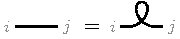
\includegraphics[scale=1.0,valign=c]{VAdelta_twisteqimon.pdf}\,,
\end{equation}
or giving one more touch,
\begin{equation}
    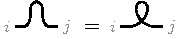
\includegraphics[scale=1.0,valign=c]{VAdelta_twisteqimon2.pdf}\,.
    \label{eq:deltatwistimon}
\end{equation}

graphically representing $\nabla_i = \partial_{i}$
can be achieved by an empty
circle, or a `balloon'. Things inside the balloon are
subjected to Leibniz-rule differentiation
\begin{align}
    \label{eq:Leibnizrule}
    {\renewcommand{\arraystretch}{1.5}
    \begin{array}{ccccc}
        \adjustbox{valign=c, scale=1}{
        \begin{tikzpicture}[]
            \node (f) [squ, draw] at (0,0) {$f$};
            \node (g) [right = 0.1cm of f] [squ, draw] {$g$};
            \node (dif) [empty] at ($(f)!0.5!(g)$) {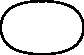
\includegraphics[scale=1.0]{CCSqBalloon9x14mm.pdf}};
            \node (tail) at ($(dif)+(0,-1.4)$) [inner sep = 2pt] {$i$}; %{\imarker{$i$}};
            \draw (dif)--(tail);
        \end{tikzpicture}
        }
        &
        =
        &
        \adjustbox{valign=c, scale=1}{
        \begin{tikzpicture}[]
            \node (f) [squ, draw] at (0,0) {$f$};
            \node (g) [right = 0.4cm of f] [squ, draw] {$g$};
            \node (dif) [circle, draw, minimum size = 9mm] at (f) {};
            \node (tail) at ($(dif)+(0,-1.4)$) [inner sep = 2pt]  {$i$}; %{\imarker{$i$}};
            \draw (dif)--(tail);
        \end{tikzpicture}
        }
        &
        +
        &
        \adjustbox{valign=c, scale=1}{
        \begin{tikzpicture}[]
            \node (f) [squ, draw] at (0,0) {$f$};
            \node (g) [right = 0.4cm of f] [squ, draw] {$g$};
            \node (dif) [circle, draw, minimum size = 9mm] at (g) {};
            \node (tail) at ($(dif)+(0,-1.4)$) [inner sep = 2pt]  {$i$}; %{\imarker{$i$}};
            \draw (dif)--(tail);
        \end{tikzpicture}
        }
        \\
        {}&{}&{\updownarrow}&{}&{}
        \\
        {\partial_i(fg)}
        &
        =
        &
        {\partial_i(f)\,g}
        &
        +
        &
        {f\,\partial_i(g)}
    \end{array}}
\end{align}
This it frequently appears as div ergence and curl:
\begin{equation}
    \adjustbox{valign=c}{\begin{tikzpicture}
        \node (shift) [empty] at (0,0.2) {};
        \node (A) [squ, draw] at (0,0) {$A$};
        \node (dif) [empty] at ($(A)+(0.04,0)$) {
\includegraphics[scale=1.0]{CCSqBalloon9mm.pdf}};
        \node (j) [empty] at ($(A)+(0,-0.95)+(shift)$) {};
        \node (i) [empty] at ($(j)+(0.45,0)$) {};
        \draw (A) to (j);
        \node (aux) [outer sep = 0] at ($(i)+(0,0.55)-(shift)$) {};
        \draw ($(dif)-(-0.35,0.3)$) ..controls(aux).. (i);
        \node (mij) [empty] at ($(i)!0.5!(j)$) {};
        \node (mb) [empty] at ($(mij)+(0,-0.225)$) {};
        \draw [rounded corners = 0.225 cm] (i) |- (mb) -| (j);
        \node (phantom) [empty] at ($(0,-0.95)+(0,-0.225)$) {};
    \end{tikzpicture}}
    \,\,=\,\,
    \nabla\cdot\vec{A}\,\,,\quad
    \adjustbox{valign=c}{\begin{tikzpicture}
        \node (shift) [empty] at (0,0.13) {};
        \node (A) [squ, draw] at (0,0) {$A$};
        \node (dif) [empty] at ($(A)-(-0.04,0)$) {
\includegraphics[scale=1.0]{CCSqBalloon9mm.pdf}};
        \node (j) [empty] at ($(A)+(0,-0.95)$) {};
        \node (xJ) [empty] at ($(A)+(0,-0.95)+(0,0.1125)$) {};
        \node (i) [empty] at ($(j)-(-0.45,0)$) {};
        \node (xI) [empty] at ($(j)-(-0.45,0)+(0,0.1125)$) {};
        \node (I) [empty] at ($(xI)+(0,0.1125)$) {};
        \node (J) [empty] at ($(xJ)+(0,0.1125)$) {};
        \draw (A) to ($(J)+(shift)$);
        \node (aux) [outer sep = 0] at ($(xI)+(0,0.55)-(0,0.1125)$) {};
        \draw ($(dif)-(-0.35,0.3)$) ..controls(aux).. ($(I)+(shift)$);
        \node (mij) [empty] at ($(i)!0.5!(j)$) {};
        \node (mb) [empty] at ($(mij)+(0,-0.225)$) {};
        \node (mijup) [empty] at ($(mij)+(shift)$) {};
        \draw (mijup)--(mb);
        \draw ($(I)+(shift)$) ..controls($(xI)-({0.01*sqrt(3)},0.01)+(shift)$)..(mijup);
        \draw ($(J)+(shift)$) ..controls($(xJ)-(-{0.01*sqrt(3)},0.01)+(shift)$)..(mijup);
        \fill [fill = black] (mijup) circle (1.3pt);
    \end{tikzpicture}}
    \,\,=\,\,
    \nabla\times\vec{A}\,\,.
    \label{eq:divcurl}
\end{equation}

Sticking only to 2 dimensions, \SOn{3} symmetry, as they do, but not
making generators unitary, $C_{ijk} = i\,\epsilon_{ijk}$ leads to an annoying
minus sign in the reduction of pair's of Levi-Civita tensors,
\begin{equation}
    \adjustbox{valign=c}{
    \begin{tikzpicture}
        \node (O) at (0,0) [empty] {};
        \node (alpha) at (0,0.2) [empty] {};
        \node (beta) at (0,-0.2) [empty] {};
        \node (xi) at ($(alpha)+(30:0.4)$) [empty] {};
        \node (xj) at ($(alpha)+(150:0.4)$) [empty] {};
        \node (xl) at ($(beta)+(-150:0.4)$) [empty] {};
        \node (xm) at ($(beta)+(-30:0.4)$) [empty] {};
        \node (i) at ($(xi)+(0,0.2)$) [empty] {};
        \node (j) at ($(xj)+(0,0.2)$) [empty] {};
        \node (l) at ($(xl)+(0,-0.2)$) [empty] {};
        \node (m) at ($(xm)+(0,-0.2)$) [empty] {};
        \fill (alpha) circle (1.3pt);
        \fill (beta) circle (1.3pt);
        \draw (alpha) -- (O) node [anchor = west] {} -- (beta);
        \draw (i) ..controls(xi).. (alpha) ..controls(xj).. (j);
        \draw (l) ..controls(xl).. (beta) ..controls(xm).. (m);
    \end{tikzpicture}}
    \,\,=\,\,
    \adjustbox{valign=c}{
    \begin{tikzpicture}
        \node (O) at (0,0) [empty] {};
        \node (alpha) at (0,0.2) [empty] {};
        \node (beta) at (0,-0.2) [empty] {};
        \node (xi) at ($(alpha)+(30:0.4)$) [empty] {};
        \node (xj) at ($(alpha)+(150:0.4)$) [empty] {};
        \node (xl) at ($(beta)+(-150:0.4)$) [empty] {};
        \node (xm) at ($(beta)+(-30:0.4)$) [empty] {};
        \node (i) at ($(xi)+(0,0.2)$) [empty] {};
        \node (j) at ($(xj)+(0,0.2)$) [empty] {};
        \node (l) at ($(xl)+(0,-0.2)$) [empty] {};
        \node (m) at ($(xm)+(0,-0.2)$) [empty] {};
        \draw (i) ..controls ($(xi)-(0,0.2)$) and ($(xl)+(0,0.2)$) .. (l);
        \draw (j) ..controls ($(xj)-(0,0.2)$) and ($(xm)+(0,0.2)$) .. (m);
    \end{tikzpicture}}
    \,\,-\,\,
    \adjustbox{valign=c}{
    \begin{tikzpicture}
        \node (O) at (0,0) [empty] {};
        \node (alpha) at (0,0.2) [empty] {};
        \node (beta) at (0,-0.2) [empty] {};
        \node (xi) at ($(alpha)+(30:0.4)$) [empty] {};
        \node (xj) at ($(alpha)+(150:0.4)$) [empty] {};
        \node (xl) at ($(beta)+(-150:0.4)$) [empty] {};
        \node (xm) at ($(beta)+(-30:0.4)$) [empty] {};
        \node (i) at ($(xi)+(0,0.2)$) [empty] {};
        \node (j) at ($(xj)+(0,0.2)$) [empty] {};
        \node (l) at ($(xl)+(0,-0.2)$) [empty] {};
        \node (m) at ($(xm)+(0,-0.2)$) [empty] {};
        \draw (i) -- (m);
        \draw (j) -- (l);
    \end{tikzpicture}}\,\,\,.
    \label{eq:theidentity}
\end{equation}
but it would be hard for them to motivate that $i$.



\item[2019-12-08 Predrag]
References collected from in Kim, Oh and Kim\rf{KiOhKi19}:

Sylvester\rf{Sylvester78} {\em On an application of the new atomic
theory to the graphical representation of the invariants and covariants
of binary quantics, with three appendices}.
Predrag wrote
``lots of blah-blah and one plate with many figures.''

Clifford\rf{Clifford1878} {\em Extract of a letter to {Mr. Sylvester}
from {Prof. Clifford} of {University College, London}}

Kempe\rf{Kempe1885}
{\em On the application of {Clifford}'s graphs to ordinary binary quantics}

Cayley\rf{Cayley1857}
{\em {XXVIII}. {On} the theory of the analytical forms called trees}

Richter-Gebert and Lebmeir\rf{RicGeb09}
{\em Diagrams, tensors and geometric reasoning}

Blinn\rf{Blinn02}
{\em Quartic discriminants and tensor invariants}

Peterson\rf{Pet06}
{\em {Trace diagrams, representations, and  low-dimensional topology}}

Peterson\rf{Pet07}
{\em A not-so-characteristic equation: the art of linear algebra}

Peterson\rf{Pet09}
{\em Unshackling linear algebra from linear notation}

Peterson\rf{Pet09a}
{\em On a diagrammatic proof of the {Cayley-Hamilton} theorem}

Morse and Peterson\rf{MorPet10}
{\em Trace diagrams, signed graph colorings, and matrix minors}

\HREF{https://arxiv.org/search/cs?searchtype=author&query=Vontobel\%2C+P+O}
{Vontobel} has many birdtrack publications.

\item[2020-09-19 Predrag]
Lifson, Reuschle and Sj{\"o}dahl\rf{LiReSj20}
{\em Introducing the chirality-flow formalism}: ``
At the algebra level, the Lorentz group consists of two copies of the
(complexified) \SUn{2} algebra [...] we
introduce the chirality-flow formalism for massless tree-level QED and
QCD, [with] scattering amplitudes
 written down in terms of Lorentz-invariant spinor inner
products, similar to how the color structure can be described in terms of
a color flow.

[...] a flow picture, similar to the color-flow picture in QCD. Recalling
the QCD Fierz identity, we analogously write the spinor Fierz identity in
a flow form. [...] the photon exchange [is] recast into a flow-like
picture [resulting in] massless tree-level QED Feynman rules. [...]
chirality-flow formalism gives a transparent and intuitive way of
understanding the Lorentz inner products appearing in scattering
amplitudes, similar to how color structure can be thought about in terms
of a color flow. [...] a simplification of the spinor-helicity
method, where Dirac spinors are replaced by their left- and right-chiral
components, and Dirac matrices by Pauli matrices. [...] we
remove the Pauli matrices as well, and instead express all
internal structure with Kronecker delta functions.
''

For details, see:
Lifson, Reuschle and Sj{\"o}dahl
{\em The chirality-flow formalism} \arXiv{2003.05877}: ``
We take a fresh look at Feynman diagrams in the spinor-helicity
formalism. Focusing on tree-level massless QED and QCD, we develop a new
and conceptually simple graphical method for their calculation. In this
pictorial method, which we dub the chirality-flow formalism, Feynman
diagrams are directly represented in terms of chirality-flow lines
corresponding to spinor inner products, without the need to resort to
intermediate algebraic manipulations. ''

\item[2020-10-19 Predrag]
Chmutov, S. and Duzhin, S. and Mostovoy\rf{ChDuMo12}
{\em Introduction to Vassiliev Knot Invariants},
\arXiv{1103.5628};
\HREF{http://www.pdmi.ras.ru/~duzhin/papers/cdbook/cdbook.pdf}
{(prepublication copy)}:

Dror Bar-Natan
\HREF{https://www.ams.org/journals/bull/2013-50-04/S0273-0979-2013-01413-7/}
{MathSci book review}:
``Vassiliev–Goussarov'' invariants %[Va1,Va2,Go1,Go2,BL,Ko1,Ko2,BN1],
which made the surprising relationship between knots and Lie algebras
appear simple and almost inevitable. Chmutov, Duzhin and
Mostovoy\rf{ChDuMo12} book is about that perspective, the one reasonable
sounding but not entirely trivial theorem that is crucially needed within
it(the Fundamental Theorem or the Kontsevich integral), and the many
threads that begin with that perspective.

The briefer summary is that in some combinatorial sense it is possible to
``differentiate'' knot invariants, and hence it makes sense to talk about
``polynomials'' on the space of knots — these are functions on the set of
knots (namely, these are knot invariants) whose sufficiently high
derivatives vanish. Such polynomials can be fairly conjectured to separate
knots — elsewhere in mathematics in lucky cases polynomials separate
points, and in our case, specific computations are encouraging.  Also,
such polynomials are determined by their ``coefficients'', and each
of these, by the one-side-easy Fundamental Theorem, is a linear functional
on some finite space of graphs modulo relations. These same graphs turn
out to parameterize formulas that make sense in a wide class of Lie
algebras, and the said relations match exactly with the relations in the
definition of a Lie algebra — anti-symmetry and the Jacobi identity. Hence
what is more or less dual to knots (invariants), is also, after passing to
the coefficients, dual to certain graphs which are more or less dual to
Lie algebras.

 \item[2020-02-13 Predrag]
 \HREF{https://www3.nd.edu/~johnson/} {Walter Johnson} writes:
Sums of products of three-j symbols over magnetic quantum numbers mj can
be formulated in terms of a set of graphical rules, that allow one to
carry out the required calculations efficiently. There are several ways
of introducing graphical rules for angular momentum summations
(Judd\rf{Judd63}; Jucys et al.\rf{YutsisLevVan62}; Varshalovich et
al.\rf{VaMoKh88}). Here, we follow those introduced by Lindgren and
Morrison\rf{LinMor82}.




\end{description}

\newpage
\section{Heisenberg algebras}
\label{s-Heisenberg}

\begin{description}

\item[2018-08-11 Predrag]
As I needed to advertise my
\HREF{http://chaosbook.org/course1/about.html} {ChaosBook} course, I was
told to do it on Twitter. Once there, I asked the heavy Twitterati
Strogatz and \HREF{https://twitter.com/johncarlosbaez} {Baez} for help,
and thus I became their follower. Baez is very enthusiastic about
categorification. I paid this no heed, but perhaps we should - it is
replete with birdtracks, the Littlewood-Richardson rule, Young projection
operators (AKA ``Young idempotents''), and such.

Categorification\rf{BaeDol98} is a process of replacing set theoretic
theorems by category-theoretic analogues. It replaces sets with
categories, functions with functors, and equations between functions by
natural transformations between functors, which in turn should satisfy
certain equations of their own called the coherence law.

Khovanov\rf{Khovanov14} {\em Heisenberg algebra and a graphical calculus},
\arXiv{1009.3295} is the foundational paper in this field.
He gives a categorification of the Heisenberg algebra that acts naturally
on the graphical category of representations  of  symmetric  group.
Abstract: ``
A new calculus of planar diagrams involving diagrammatics for biadjoint
functors and degenerate affine Hecke algebras is introduced. The calculus
leads to an additive monoidal category whose Grothendieck ring contains
an integral form of the Heisenberg algebra in infinitely many variables.
We construct bases of vector spaces of morphisms between products of
generating objects in this category.
''

Khovanov\rf{Khovanov14} work is discussed in length by
Gonz{\'a}lez\rf{Gonzalez18} {\em Categorical {Bernstein} operators and the
{Boson-Fermion} correspondence}, \arXiv{1808.01235},
which seems to be (a part of?)
\HREF{https://sites.google.com/usc.edu/nicollesandovalgonzalez/}
{Nicolle Sandoval Gonz{\'a}lez} PhD thesis. She uses our Young idempotents,
which is why I got bogged down in reading this literature. Here is her
\HREF{http://www.dtubbenhauer.com/Gonzalez.pdf} {2017 talk}.

Licata and Savage\rf{LicSav13} {\em Hecke algebras, finite general linear
groups, and {Heisenberg } categorification}, \arXiv{1101.0420}

Licata and Savage\rf{LicSav11} {\em A survey of {Heisenberg}
categorification via graphical calculus},
\arXiv{1104.4789}. I cannot reach the published version
Bull. Inst. Math. Acad. Sin. (N.S.) 7 (2012), pp. 291--321
at \HREF{http://www.math.sinica.edu.tw/} {www.math.sinica.edu.tw};
the Great Wall of China in action?

Cai, Lin and Wu\rf{CaiLiWu12}
{\em A diagrammatic categorification of q-boson and q-fermion algebras}

Cooper and Hogancamp\rf{CooHog15}
{\em An exceptional collection for {Khovanov} homology} uses
Jones–Wenzl projectors; Temperley–Lieb, ...

Hill and Sussan\rf{HillSus16} {\em A categorification of twisted
{Heisenberg} algebras}
replace the symmetric group with its superversion - the Hecke–Clifford
algebra.

%Abel and Hogancamp\rf{AbelHog17} {\em Categorified {Young symmetrizers}
%and stable homology of torus links {II}}
% lots of projection operators; no birdtracks

Brundan\rf{Brundan17} {\em On the definition of {Heisenberg} category}

Licata, Rosso and Savage\rf{LiRoSa18} {\em A graphical calculus for the
{Jack} inner product on symmetric functions}: ``It would be interesting to
give a graphical description of the Jack symmetric functions.''

The antisymmetric property of fermions in physics can be understood in
the framework of differential graded categories.
Lipshitz \etal\rf{LiOzTh18} {\em Bordered Heegaard Floer homology:
invariance and pairing} define a diagrammatic differential graded
algebra, called the strands algebra in the context of bordered Heegaard
Floer homology.

Savage\rf{Savage18} {\em String diagrams and categorification}


\end{description}

\Remarks

\remark{Birdtracks.}{\label{rem:birdtrHist}
The history of birdtracks as of 2004 is discussed in
Sec.~4.9 of {\em Group Theory: Birdtracks, Lie's and Exceptional Groups}\rf{PCgr}.
Here are some further remarks, mostly based on 2017 Keppeler\rf{Keppeler17}.

%\item[2003-02-05  ] %<srinivas@uic.edu>
\HREF{https://en.wikipedia.org/wiki/Bhama_Srinivasan} {Bhama}
\HREF{http://www-history.mcs.st-andrews.ac.uk/Biographies/Srinivasan.html}
{Srinivasan} credits R. Brauer {\em On algebras which are connected with
the semisimple continuous groups}\rf{Brauer1937} for an early use of
diagrammatic notation, in 1937. The algebra Brauer constructed is now
called the Brauer algebra (essentially birdtracks for SO/Sp:1), but
people now study it algebraically.
% I had a student who worked on it and found a nice
% basis for it in his Ph.D thesis.

% \item[2017-07-23 Keppeler's further reading]

Roger Penrose introduced birdtracks (or fornicating ostriches, as one of
his colleagues prefers to call them) in 1952 in order to describe tensors in
general relativity. A good introduction is his
  ``popular'' science book {\it The Road to Reality}\rf{Penr04}. There,
  birdtrack diagrams are introduced in Sects.~\S12.8, \S13.3--\S13.9,
  \S14.3, \S14.4, \S14.6, and \S14.7 in the context of differential
  geometry and later (Secs.~\S19.2, \S19.6, \S22.12, \S26.2, \S29.5)
  used for general relativity and other topics.

The 1976 Cvitanovi{\'c} paper\rf{PCar} provides an
  introduction and summary of birdtracks for $\SUn{N}$ and QCD.

The 1990 book {\it Diagram Techniques in Group Theory} by Geoffrey
  E. Stedman\rf{StedmanBook} also treats many aspects and applications
  of the birdtrack method; it also contains an introductory
  section on vector algebra.

Yuri L.\ Dokshitzer's 1995 lecture notes\rf{DokSchSlo97} {\it Perturbative QCD (and
    beyond)} introduces birdtrack techniques using
  QCD processes as examples; some of his notational conventions differ
  slightly from ours.

Young operators (non-Hermitian) in birdtracks are discussed in
 \refref{YoungUn}.

The main references for the construction of multiplet bases are
 \refrefs{KeppSjo12,KeppSjo14}. Hermitian Young operators are constructed
  in \refref{KeppSjo14}, gluon projectors and the general rules for
  constructing multiplet bases are derived in \refref{KeppSjo12}.
  Hermitian Young operators and multiplet basis for few quarks appear
  already in \refrefs{NPB81, Canning1978ee, PCgr}. The multiplet basis for
  $A^{\otimes 2}\to A^{\otimes 2}$ in birdtracks is constructed in
 \refref{PCgr} using a different method.
  Simplification rules for a more efficient construction of Hermitian
  Young operators are derived in \refrefs{AlcZei16-1,AlcZei16-2}. The
  corresponding quark multiplet bases are discussed in
 \refref{AlcZei16-3}.

Sj{\"o}dahl and co-workers discuss decomposition into multiplet
  bases\rf{SjoTho15} and recursion relations\rf{DuSjoTho15}.

A birdtracks cheat sheet: App.~A of \refref{KeppSjo12}.
When pen and paper calculations become unwieldy, the Mathematica and {\tt
C++} packages\rf{Sjodahl13,Sjodahl15} by Malin Sj{\"o}dahl come in handy.
All birdtracks in
\refref{Keppeler17} where typeset with {\tt JaxoDraw}\rf{BinThe04}.

\hfill P. Cvitanovi{\'c} and S. Keppeler
} % end \remark{Birdtracks.}{\label{rem:birdtrHist}

\remark{Group theory background.}{\label{rem:background}
Classic results on the representation theory of finite groups (such as
$\textrm{S}_n$) and compact Lie groups (such as $\SUn{N}$), on Schur's lemma, or
on the multiplication of Young diagrams can, e.g., be found in
Hamermesh\rf{Hamermesh1962},
Tung\rf{Tung1985na},
Simon\rf{Sim96},
and in a vast number of other textbooks.

\hfill P. Cvitanovi{\'c} and S. Keppeler
    }% \remark{Background.}{\label{rem:background}

\RemarksEnd

%\newpage %%%%%%%%%%%%%%%%%%%%%%%%%%%%%%%%%%%%%%%%%%%%%%%%
\printbibliography[heading=subbibintoc,title={References}]
